\section{Overview}
%URN构主要由vRNIC(前端和后端)和URN core两大部分组成。vRNIC是一个半虚拟化的RDMA网卡设备,每个vRNIC都有一对前后端,通过前后端的交互为guest提供虚拟的RDMA服务;URN 是对vRNIC虚拟RDMA的管理模块。此外,对host和容器的verbs进行了修改以以便与URN框架协作。
The architecture of URN is shown in Figure~\ref{fig:framework-overview}. URN mainly consists of vRNIC (virtual RDMA interface card) and URN core. The vRNIC is a para-virtualization virtual device for guest, which includes a pair of frontend and backend; the URN core is a manageable unit for different vRNICs in each host. Besides, some modifications are made to host's  verbs libraries and containers' verbs libraries  for cooperating with URN.

% (1) vRNIC Frontend(FE): FE位于guest,是一个虚拟的RDMA网卡接口提供给上层verbs。Guest应用可以通过verbs库直接使用FE。在虚拟机里,FE在guest内核,通过与原RDMA内核驱动一致的接口与verbs库交互;在容器里,FE是一个用户库,容器应用使用修改的verbs库时链接FE,并通过定制化的接口与FE交互,该过程无需再陷入到主机内核。
(1) vRNIC Frontend: locates in guest, as the interface of vRNIC. Guests' applications can use the vRNIC interface through verbs libraries. For VMs, the frontend is in guest kernel and designed same as native interface for upper unmodified verbs; For containers, the frontend is a library for upper modified verbs linking. Thus, the interacts between container verbs and vRNIC frontend are still in user space, not in kernel.

% (2) vRNIC Backend(BE): BE位于host的用户空间,是vRNIC的虚拟设备后端。BE虚拟化了所有的RDMA网卡属性,例如QP。BE通过URN Core进行实例化,并通过修改过的Verbs库与RDMA物理网卡交互,维持RDMA上下文并提供给FE。在RDMA控制路径,BE和通常半虚拟化一致,执行FE转发的操作并返回给FE。在数据路径,应用直接在guest用户空间使用已经与BE映射的RDMA资源。
(2) vRNIC Backend: locates in host user-space. vRNIC backend is virtual device backend, which has virtualized basic RDMA attributes, e.g. QP, MR. Backends are inited through the URN core and interact with physical RNIC by verbs libraries. RDMA contexts are maintained in backends for the requests from frontends. In specific, in data path, the backends provided mapped RDMA resources for applications in guest, e.g. QPs and MRs, and guest applications can directly use them locally.

%(3)URN core:每台主机都有一个URNC core位于用户空间, 负责管理本地的RDMA虚拟网络,包括实例化BE、映射虚拟RDMA连接和配置路由等。URN core与修改过的Verbs用户库交互,再通过原生RDMA内核驱动实现对RDMA网卡的控制。
(3) URN core: There is a UNR core in each host's user-space. URN core is designed to manage the virtual RDMA network for each host, including initing vRNIC backends, mapping virtual RDMA connections and configuring rules. URN core also interact with physical RNIC through verbs libraries. 

% 此外,,本文对容器的verbs库和主机verbs库进行了少量修改。在容器的修改,让Verbs库可以直接在用户空间与FE交互, 不用经过主机内核。在主机的修改,以支持RDMA后端使用共享内存对QP和MR等资源进行映射。为了实现与应用程序的透明性,上述修改均未破坏RDMA应用与Verbs库的API。
Besides,  we modified the verbs libraries in containers,  the RDMA verbs can be forwarded to vRNIC frontends, instead of host kernel. Also, we modified the verbs libraries in host, to support mapping RDMA resources through shared memory in vRNIC backends. Note that all modifications are inside the internal, and do not change the verbs API in guest. Thus, URN is still transparent for guest applications.

\begin{figure}[!ht]
	\centering
	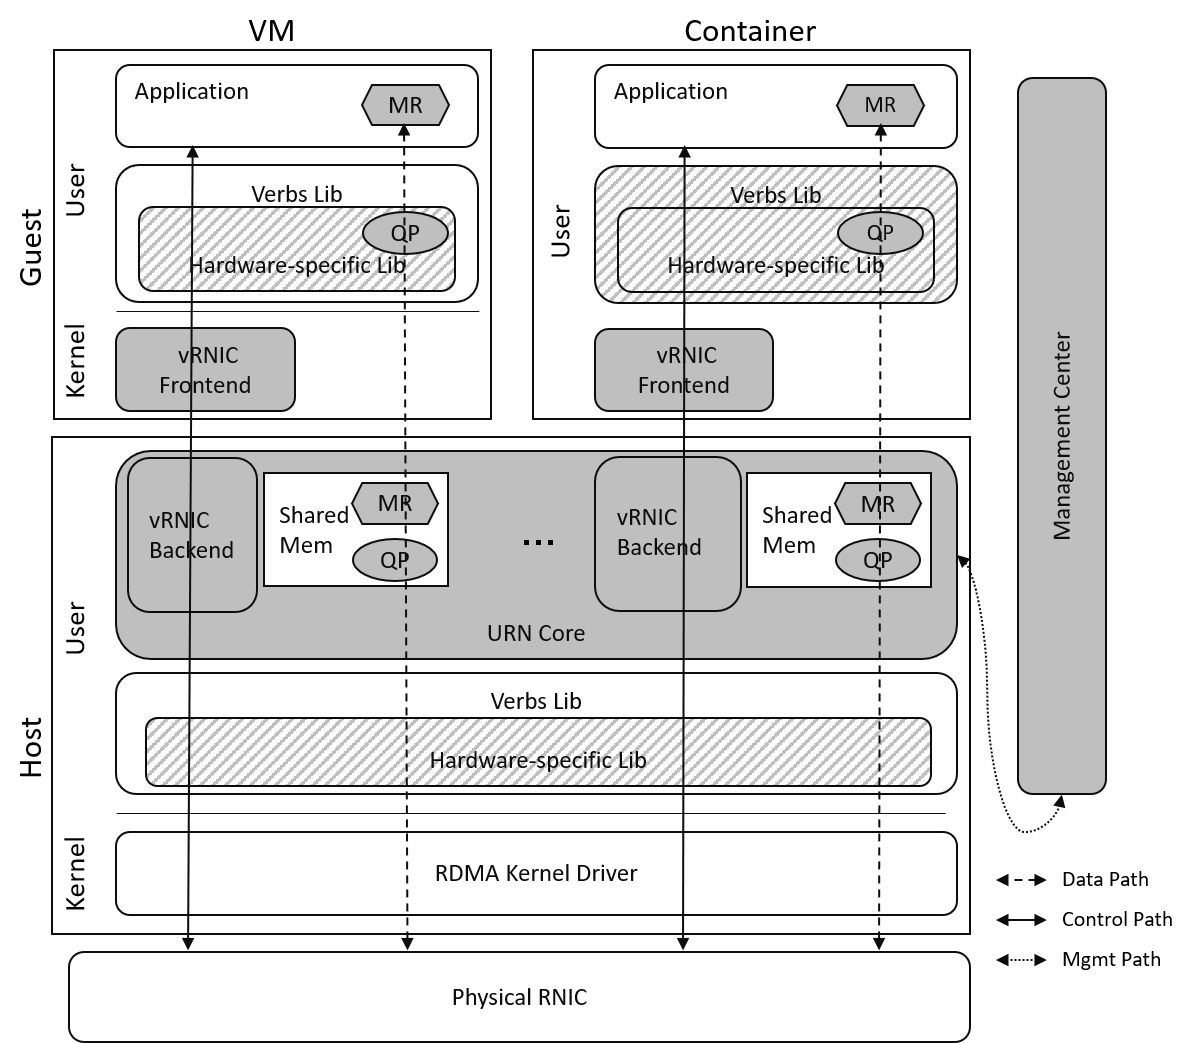
\includegraphics[width=1\linewidth]{images/framework-overview.png}
	\caption{uniRDMA Framework Overview}
	\label{fig:framework-overview}
\end{figure}